\documentclass{article}

% See http://mirror.its.dal.ca/ctan/macros/latex/contrib/appendix/appendix.pdf for more appendix info
\usepackage[page,toc,title,titletoc]{appendix}
\usepackage[
	backend=bibtex,
	natbib=true,
	style=numeric,
	sorting=none
]{biblatex}
\usepackage{graphicx}
\usepackage{lipsum}
\usepackage{pgfgantt}

% Temporary bugfix for BibTeX
% Found at http://tex.stackexchange.com/a/311428
\makeatletter
\def\blx@maxline{77}
\makeatother

\bibliography{proposal}

\title{Fourth Year Project Proposal}
\author{
	Craig Shorrocks \\
	100887781
	\and
	Jessica Morris \\
	100882290
	\and
	Richard Perryman \\
	100887250
}

% Might be better to use the last date we edit this on,
% but for now I was too lazy to keep updating this
\date{\today}

\begin{document}

\maketitle

\begin{center}
Supervisors: Shikharesh Majumdar and Chung-Horng Lung
\end{center}

\pagebreak

\tableofcontents

\pagebreak

\section{Objective}

As technology becomes more and more prevalent in our lives, our identities become more and more intertwined with the
technologies that we use daily. This melding has become extremely prevalent in some areas. Some such areas are
professional networking with LinkedIn, or banking with the advent of online account management. Over half of all
smartphone users have used mobile banking~\autocite{MOBILEBANKING}. This popularity may be derived
from how convenient and secure handling money online is. However, certain aspects of our day to day lives haven't yet
been graced by the benefits of electronic security and automation.

Physical locks and keys are still widely used for several tasks where electronic locks could be used instead. House
locks, bicycle locks, and locker locks are frequently physical locks. Changing to electronic locks could help streamline
all of these locks, reducing the number of keys to remember and improving security by reducing the likelihood that the
key could be faked by an attacker. Some applications for this have already been found: for example, Walmart has a
system where customers can order products to be placed in lockers with electronic keys called
Grab-and-Go~\autocite{WALMART}. Such a system greatly reduces the work involved in getting a key (in this case, a
PIN instead of a physical key or combination) to the customer and increases the security of the lockers by reducing the number
of points of failure.

This proposal outlines a system that will expand upon such a concept to further tie security and identity to the
electronics we use most: our phones. Using technologies like near-field communication (NFC) sensors and quick response
(QR) codes, the identity associated with a phone can be used as identification for anything. This represents a huge
advantage with respect to convenience, and it would even further lower the number of possible failure points in
security.

\section{Background}

NFC is a form of short-range, low-power communication used by devices such as smartphones, and tablets. NFC is a fast
and convenient method to exchange small amounts of data, as it does not require any steps to set up a connection. One
device, the active device, uses magnetic induction to induce a current in the information-holding "passive device". The
passive device responds by modulating the EM field coming from the active device, and the active device converts the
modulations into useful data~\autocite{NFCORG}. This scenario is a NFC communication in passive mode. Two smartphones
may both act as passive and active devices, allowing them to exchange data through a call-and-response procedure, also
known as communication in active mode.

NFC is being increasingly used to "smarten up" passive information delivery systems such as business cards, and posters.
Information such as contact information, URLs, or credentials may be written to a passive NFC device, such as a smart
tag~\autocite{NFCFORUMWHATIS}, and read by any NFC-enabled mobile device. These mobile devices can also be used to
replace credit cards in contactless exchanges. In fact, NFC payments may be more secure than payment with a card, as
each point in the transaction requires the device and the reader to exchange an encrypted password, and the transactio
 must be approved by the device's user before the device sends payment information~\autocite{NFCPAYMENT}.

Because of the close range required for an exchange, NFC has inherent protections against attackers. An NFC exchange
can only be reliably eavesdropped from a distance of approximately 10 m or less if the interaction is between two active
devices, dropping to 1 m if the interaction is a passive communication; and a man-in-the-middle attack is nearly
impossible to accomplish in a real-world scenario \autocite{NFCSECURITY}. These attacks may be protected against by
establishing a secure channel, by using symmetric-key encryption or other secret-sharing method. For these reasons,
NFC is a reliable method to pair a smart device with an electronic lock.

\section{Methods}

% Buzzwords FRAMEWORK buzzwords
% Authentication token established at access
% OAuth - restful services
% Refer to use case diagram in appendix
% Refer to block diagram

\lipsum[1]

\section{Time Table}

% Should timeline start from week of Sept 9?
% Prepare Proposal
% Preliminary design
% Preliminary testing
% Integrate soft/hardware
% Integration testing
% December 9th 2016 - Progress Report
% January 23rd 2017 - Saturday, January 28th 2017 - Oral Presentations
% March 20th 2017 - Poster Fair
% April 7th 2017 - Final Report due

\lipsum[1]

\section{Components}

\begin{itemize}
	\item Raspberry Pi 3 Model B with 5V power supply and microSD card
	\item Rasperry Pi Camera NoIR Board Add-on
	\item Adafruit Feather 32u4 FONA with prototyping board
	\item Starter Pack for Arduino (with Arduino Uno R3)
	\item Adafruit PN532 NFC shield
	\item Soldering tools in ME4135
	\item Amazon Web Services - Amazon API Gateway, Amazon RDS
\end{itemize}

\pagebreak

\begin{appendices}

\section{UML}

\begin{figure}[!ht]
	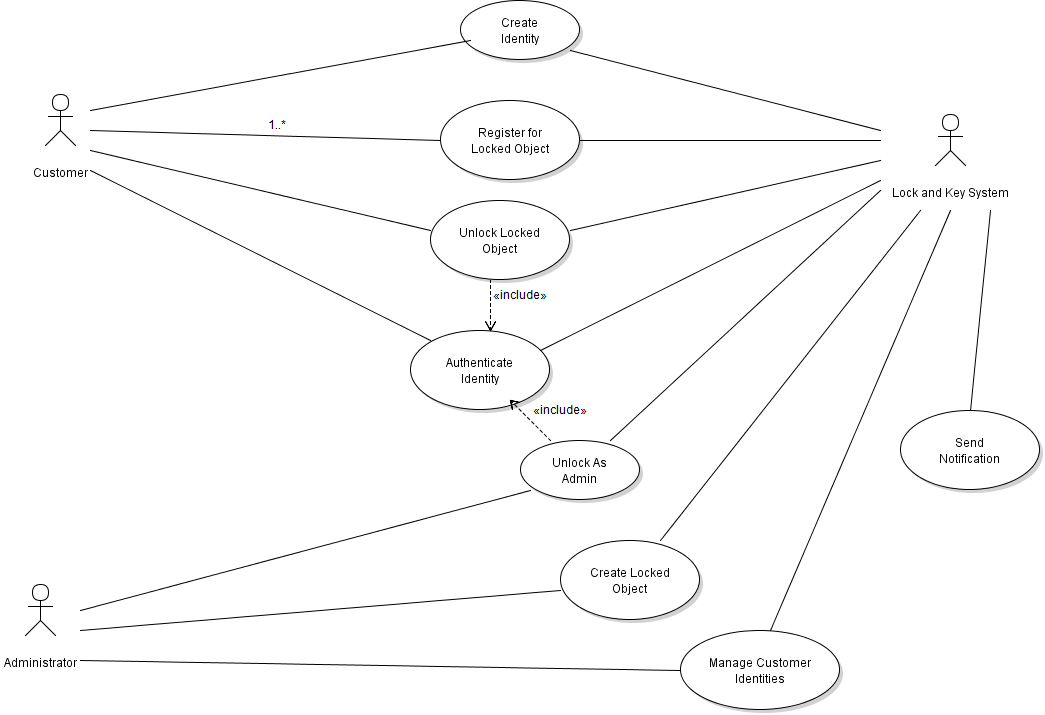
\includegraphics[width=\textwidth]{UML/lock_and_key}
	\caption{Use case diagram}
	\label{fig:use_case}
\end{figure}

\end{appendices}

\pagebreak

\printbibliography

\end{document}
\grid
